\chapter{Results} \label{Results}

\section{Evaluation methodology}

In this chapter, we will be presenting and evaluating the results yielded by our simulation. As stated in more detail in chapter \ref{Implementation}, the scenario that we are implementing here is that of a highly dense urban environment. Points are distributed according to a homogeneous PPP (section \ref{PPP}) in a set Manhattan grid (\ref{mh_grid}). Pathloss between two points accounts for both the topology of the grid as well as spatially-correlated shadow fading (\ref{SF}). Clusters are created according to the specifications of various clustering schemes (\ref{ClusteringAlgs}) and then the resulting traffic is simulated with a random access procedure at the assigned cluster heads (\ref{RAP}), where both noise and interference are accounted for.

All parameters utilized in our simulation are gathered in the two tables below, separated into those relevant for the calculation of pathloss (table \ref{tbl:PL}) and those relevant for random access and interference simulation (table \ref{tbl:RA}).

\begin{table}
\begin{center}
 \begin{tabular}{||p{10.5cm}|p{2.5cm}||} 
 \hline
 \textbf{Parameter} & \multicolumn{1}{|c||}{\textbf{Value}}\\
 \hline
 \multicolumn{2}{c}{} \\[-0.7em]
 \hline
 \multicolumn{2}{||c||}{\textbf{PPP}} \\
 \hline
 Mean point density $\lambda$ (range) & \multicolumn{1}{|c||}{$50 - 1000$} \\ 
 \hline
 \multicolumn{2}{c}{} \\[-0.7em]
 \hline
 \multicolumn{2}{||c||}{\textbf{Pathloss}} \\
 \hline
 Center Frequency $f_c$& \multicolumn{1}{|c||}{$2\,\text{GHz}$} \\
 \hline
 Wavelength $\lambda_{WL}$ & \multicolumn{1}{|c||}{$0.15\,\text{m}$}\\
 \hline
 Speed of light $c$ & \multicolumn{1}{|c||}{$3 \cdot 10^8\,\frac{\text{m}}{\text{s}}$}\\
 \hline
 Height of UE $h_{UE}$ & \multicolumn{1}{|c||}{$1.5\,\text{m}$} \\
 \hline
 Height of BS $h_{BS}$ & \multicolumn{1}{|c||}{$10\,\text{m}$} \\
 \hline
 Environment height $h_e$ & \multicolumn{1}{|c||}{$1\,\text{m}$} \\
 \hline
 Power decay constant $n_1$ & \multicolumn{1}{|c||}{$2.2\,\text{dB}$}\\
 \hline
 Power decay constant $n_2$ & \multicolumn{1}{|c||}{$4.0\,\text{dB}$}\\
 \hline
 \multicolumn{2}{c}{} \\[-0.7em]
 \hline
 \multicolumn{2}{||c||}{\textbf{Shadow Fading}} \\
 \hline
 Shadow Fading mean $\mu_{L_s}$ &\multicolumn{1}{|c||}{$0\,\text{dB}$} \\
 \hline
 Shadow Fading standard deviation $\sigma_{L_s}$ & \multicolumn{1}{|c||}{$7\,\text{dB}$}\\
 \hline
 Decorrelation distance $d_{corr}$ &\multicolumn{1}{|c||}{$8\,\text{m}$}\\
 \hline
\end{tabular}
\end{center}
\caption{Parameters relevant for pathloss calculation}
\label{tbl:PL}
\end{table}

\begin{table}
\begin{center}
 \begin{tabular}{||p{10.5cm}|p{2.5cm}||} 
 \hline
 \textbf{Parameter} & \multicolumn{1}{|c||}{\textbf{Value}}\\
 \hline
 \multicolumn{2}{c}{} \\[-0.7em]
 \hline
 \multicolumn{2}{||c||}{\textbf{Request creation \& transmission}} \\
 \hline
 Request arrival rate $\lambda_A$ & \multicolumn{1}{|c||}{$1.5$} \\ 
 \hline
 Maximum connection attempts & \multicolumn{1}{|c||}{$20$} \\ 
 \hline
 Transmission power $P_{Tx}$& \multicolumn{1}{|c||}{$23\,\text{dBm}$} \\
 \hline
 \multicolumn{2}{c}{} \\[-0.7em]
 \hline
 \multicolumn{2}{||c||}{\textbf{Noise}} \\
 \hline
 Noise density $N_0$ & \multicolumn{1}{|c||}{$-174\,\frac{\text{dBm}}{\text{Hz}}$}\\
 \hline
 UE receiver noise figure $NF_{UE}$ & \multicolumn{1}{|c||}{$9\,\text{dB}$}\\
 \hline
 BS receiver noise figure $NF_{BS}$ & \multicolumn{1}{|c||}{$5\,\text{dB}$} \\
 \hline
 System Bandwidth $W$ & \multicolumn{1}{|c||}{$10\,\text{MHz}$} \\
 \hline
 \multicolumn{2}{c}{} \\[-0.7em]
 \hline
 \multicolumn{2}{||c||}{\textbf{Interference}} \\
 \hline
 Number of total LTE-A preambles & \multicolumn{1}{|c||}{$64$} \\
 \hline
 Number of preambles available for D2D communication $m$& \multicolumn{1}{|c||}{$6$}\\
 \hline
 SINR threshold $SINR_{thr}$ & \multicolumn{1}{|c||}{$10\,\text{dB}$}\\
 \hline
 Slot duration $T_{slot}$ & \multicolumn{1}{|c||}{$10\,\text{ms}$}\\
 \hline
 Total duration $T_{total}$ &\multicolumn{1}{|c||}{$5\,\text{s}$}\\
 \hline
\end{tabular}
\end{center}
\caption{Parameters relevant for random access and interference}
\label{tbl:RA}
\end{table}

The central element that testing will be looking at is how the chosen clustering algorithms behave under varying degrees of mean UE density $\lambda$. In the case of LEACH, due to CH selection probability $P_{LEACH}$ also being a relevant parameter, we will also test for a range of values. 

Regarding the metrics used for comparison of adequacy of the different clustering schemes, we managed to narrow them down to four criteria:

\begin{itemize}
\item Percentage of UEs connecting to eNB
\item Mean channel utilization rate
\item Total resource efficiency
\item Mean UE drop ratio
\end{itemize}

In the following, we will shortly justify and explain each metric.

\subsection{Percentage of UEs connecting to eNB}
One of the original motivations behind the expansion of LTE-A through D2D proximity services is the alleviation of the load experienced by the available infrastructure with large numbers of devices. By measuring the percentage of UEs connecting directly to the eNB, we seek to quantify to what extent the given algorithm is actually reducing the traffic at the eNB.

We denote as $P_{UE\rightarrow eNB}$ and define it as
\begin{equation}\label{eq:con_eNB}
P_{UE\rightarrow eNB} = \frac {\text{UEs without cluster assignment}}{\text{Total UEs in grid}}\,,
\end{equation}
with UEs without cluster assignment meaning those that are neither transmitting to a cluster head nor are one themselves.

It is important to note here that this measure, as with all presented in this work, is not unambiguous. A very small $P_{UE\rightarrow eNB}$ may look good from the point of view of the amount of connections at the eNB, but it may belie overly large clusters that only transfer the overload problem from the base station to the individual cluster heads.

\subsection{Mean channel utilization rate}
Throughput is often used in communication networks as a measure of the amount of data being transmitted in a given time frame. In a similar vein, our measure of mean channel utilization rate, measured at individual cluster heads and then averaged over them, intends to quantify to what extent the available channel is being utilized to its full potential.

The definition given here for mean channel utilization rate $\varrho$ was proposed by this work's supervisor and is defined as
\begin{equation}\label{eq:TP}
\varrho_{channel} = \frac{N_{successes}}{m\cdot N_{slots}}\,\text{,}
\end{equation}
with $N_{successes}$ being the amount of successful connections that have been established with the cluster head, $m$ the number of preambles available for transmission (cf. section \ref{RAP}) and $N_{slots}$ the number of available time slots for transmission (see equation \ref{eq:N_slots}).
\begin{equation}\label{eq:N_slots}
N_{slots} = \frac {T_{total}} {T_{slot}} -1
\end{equation}

The final mean channel utilization rate $\overline{\varrho}_{channel}$ is then averaged out over all cluster heads.

It is worth noting how remarkably small the resulting values are for $\overline{\varrho}_{channel}$ across all measurements: this is mostly due to the way we defined the metric in the first place. Firstly, the fixed arrival rate of requests to the CH, $\lambda_A$ is kept constant at a low value of $1.5$, which automatically lowers the amount of \textit{successful} requests $N_successes$. This is of course compounded by the fact that, with a $T_{total} = 5\,\text{s}$ and a $T_{slot} = 0.01\,\text{s}$, $N_{slots}$ evaluates to $500$. 

\subsection{Total resource efficiency}\label{RE}
The inclusion of resource efficiency as a metric was born out of a desire to have a measure that somewhat quantified the potential gains that the expansion of LTE-A into D2D communication can have. To this effect, we looked into the work presented in \cite{Klugel2014}, where it is sought to introduce a measure for efficiency in D2D communications. The authors, recognizing how traditional measures such as throughput, do not accurately reflect the gains of D2D, propose a measure of resource efficiency for the whole network $RE(\mathcal{G})$ based on the available resources it uses:
\begin{equation}\label{eq:RE}
RE(\mathcal{G}) = \sum_{w_{ij}\in\mathcal{W}}\eta_{ij}RE(w_{ij})\,\text{.}
\end{equation}
In the above equation, $\eta_{ij}$ is the fraction of resources $r(w_{ij})$ used out of the total resource pool $\mathcal{R(G)}$ by a link $w_{ij}$ out of all links $\mathcal{W}$
\begin{equation}\label{eq:RE2}
\eta_{ij} = \frac {|r(w_{ij})|}{|\mathcal{R(G)}|}
\end{equation}
and $RE(w_{ij})$ is the efficiency of the individual link $w_{ij}$
\begin{equation}\label{eq:RE3}
RE(w_{ij}) = \frac {TP(w_{ij})\cdot T_{total}}{|r(w_{ij})|}\,\text{,}
\end{equation}
measured with help of the link throughput $TP(w_{ij})$, the total observed time length $T_{total}$ (cf. section \ref{RAP}). Total resource efficiency given in $\frac{\text{bit}}{\text{s}\cdot\text{Hz}}$.

The total resource pool $\mathcal{R(G)}$ we define, similarly to \cite{Klugel2014} as the Cartesian product $\mathcal{R\,=\,T\,\times\,F}$ of available time $\mathcal(T)$ and frequency ($\mathcal{F}$) resources. We eschew a definition of available area resources $\mathcal{A}$ due to the difficulty of defining them in this context, an issue acknowledged by the authors, who also exclude it in their examples.

\subsection{Mean UE drop ratio}
Finally, we include a measure to quantify how successful a given device is in transmitting the information it has to. To do this, we look at the amount of times it ``is dropped'' by its respective cluster head, meaning all the times the ``back off'' limit is reached (see section \ref{RAP}). We then compare it to all attempts, both failures and successes:

\begin{equation}\label{eq:UEDR}
\theta_{drops} = \frac {\text{Number of Failures}} {\text{Number of Successes} + \text{Number of Failures}} \,\text{.}
\end{equation}

We then average this across all UEs communicating through D2D to find the final mean UE drop ratio $\overline{\theta}_{drops}$.

\section{LEACH}\label{description:LEACH}
As stated in the previous chapter, LEACH was of particular interest to us due to the influence it had had on so many other clustering algorithms in the field of WSNs (see section \ref{LEACH}), as well as the simplicity it presented. The presence of not only the expected point density $\lambda$ but also the cluster head activation probability $P_{LEACH}$ raised many questions about how the network would react to changes in both. We accordingly expanded the range of $\lambda$ of our simulation from the usual $[50 - 500]$ to $[50 - 1000]$. The overall results can be appreciated in figure \ref{fig:pretty_results_LEACH}. In the following, all figures are presented with a confidence interval, when existing, of 85\%.

\begin{figure}
  \begin{subfigure}[b]{0.5\linewidth}
    \centering
    \captionsetup{justification=centering}
    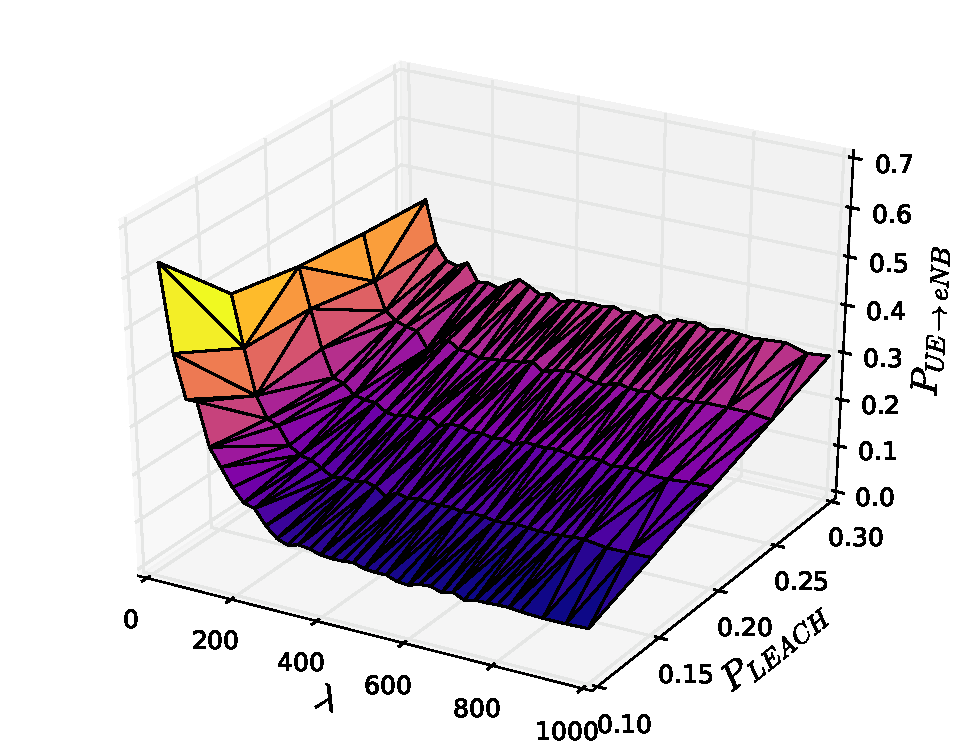
\includegraphics[width=1\linewidth]{figures/LEACH_2} 
    \caption{\% of UEs connecting to eNB $P_{UE\rightarrow eNB}$ }
    \label{fig:LEACH_2} 
    \vspace{4ex}
  \end{subfigure}%% 
  \begin{subfigure}[b]{0.5\linewidth}
    \centering
    \captionsetup{justification=centering}
    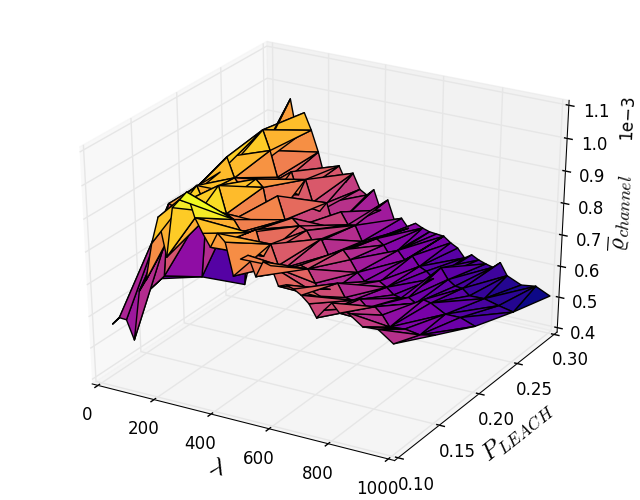
\includegraphics[width=1\linewidth]{figures/LEACH_8} 
    \caption{Mean channel utilization rate $\overline{\varrho}_{channel}$} 
    \label{fig:LEACH_8} 
    \vspace{4ex}
  \end{subfigure} 
  \begin{subfigure}[b]{0.5\linewidth}
    \centering
    \captionsetup{justification=centering}
    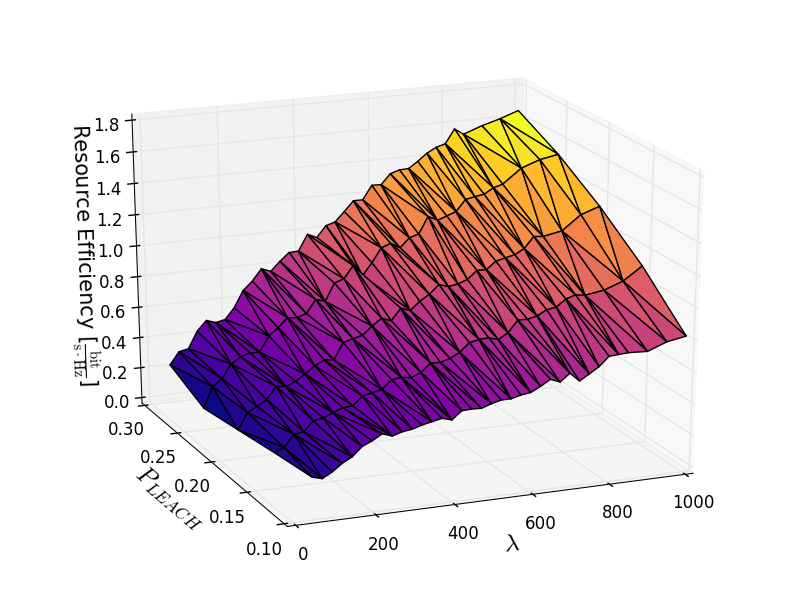
\includegraphics[width=1\linewidth]{figures/LEACH_9} 
    \caption{Total resource efficiency} 
    \label{fig:LEACH_9} 
  \end{subfigure}%%
  \begin{subfigure}[b]{0.5\linewidth}
    \centering
    \captionsetup{justification=centering}
    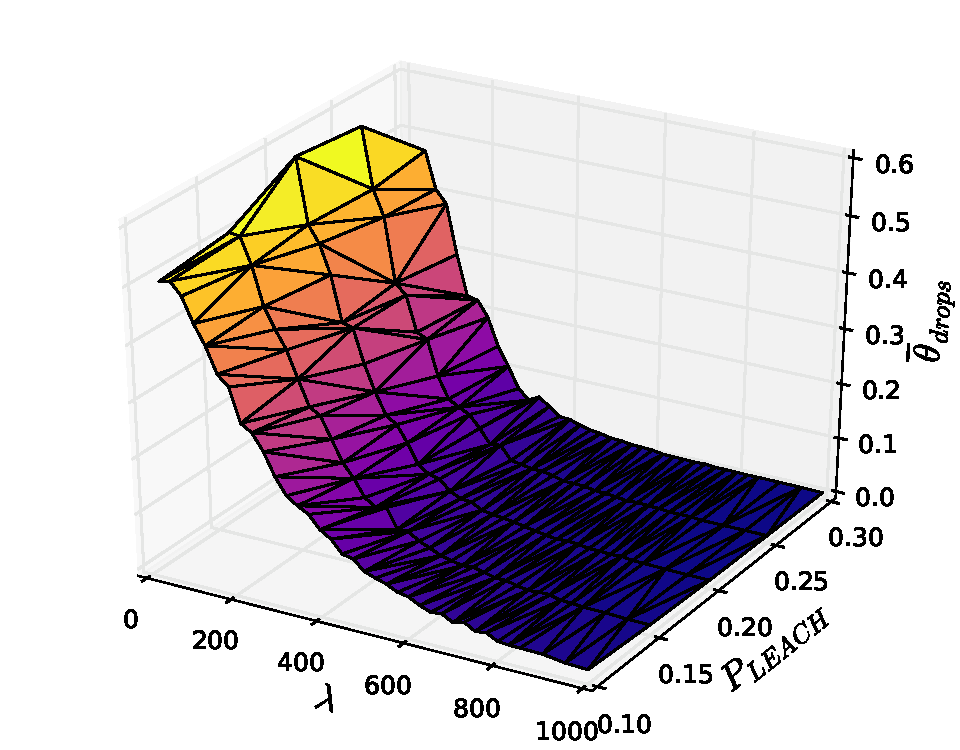
\includegraphics[width=1\linewidth]{figures/LEACH_10} 
    \caption{Mean UE drop ratio $\overline{\theta}_{drops}$} 
    \label{fig:LEACH_10} 
  \end{subfigure} 
  \caption{Behavior of LEACH compared to $P_{LEACH}$ and $\lambda$}
  \label{fig:pretty_results_LEACH} 
\end{figure}

Regarding the \textbf{percentage of UEs connecting to eNB $P_{UE\rightarrow eNB}$} (figure \ref{fig:LEACHLINES_2}), after an initial sharp increase, it goes down steadily, leveling out starting around the $\lambda = 400$ mark (see figure \ref{fig:LEACHLINES_2}). This ``final'' value is closely correlated to the cluster head activation probability $P_{LEACH}$: for $P_{LEACH} = 0.1$, $P_{UE\rightarrow eNB}$ saturates around the $10\%$ mark, for $P_{LEACH} = 0.3$, $P_{UE\rightarrow eNB}$ it moves towards $30\%$, etc. 

\begin{figure}
\centering
\captionsetup{justification=centering}
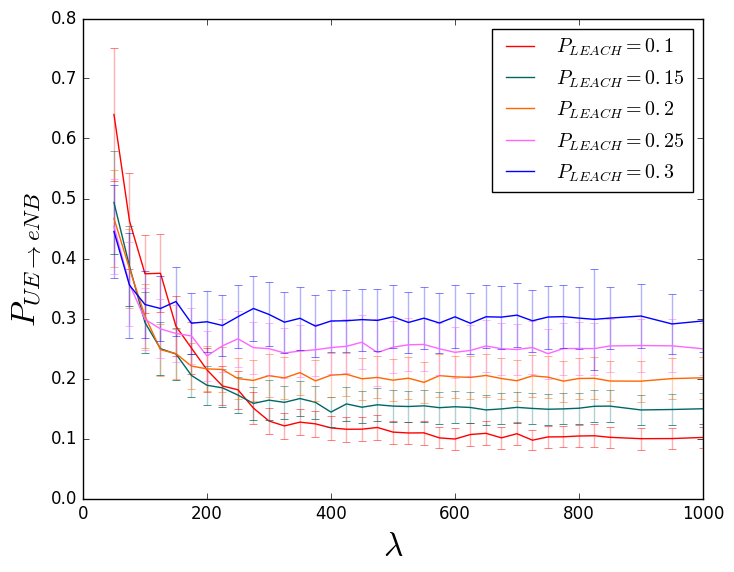
\includegraphics[width=0.7\linewidth]{figures/LEACHLINES_2}
\caption{LEACH: Percentage of UEs connecting to eNB $P_{UE\rightarrow eNB}$ in relation to mean point density $\lambda$ }
\label{fig:LEACHLINES_2}
\end{figure}

This is of course, expected behavior. The initial increase in $P_{UE\rightarrow eNB}$ can be explained by insufficient device density: having no viable cluster heads around them, devices elect to transmit their data through other means and not through D2D. Once a high enough concentration of UEs, and consequently of cluster heads is available, most UEs are able to connect to a cluster head in their vicinity. The only UEs left to transmit directly to the eNB are, of course, the cluster heads themselves.

It should be noted that $P_{UE\rightarrow eNB}$ is a \textit{percentage} and scales with absolute numbers. while $10\%$ seems like a small value, with a mean point density of, say, $700$, it means around 70 devices trying to gain access the eNB's resources. Even after data aggregation, a very high $\lambda$ means placing an inordinate amount of pressure on the available PUSCH resources.

% \begin{figure}
% \centering
% \captionsetup{justification=centering}
% 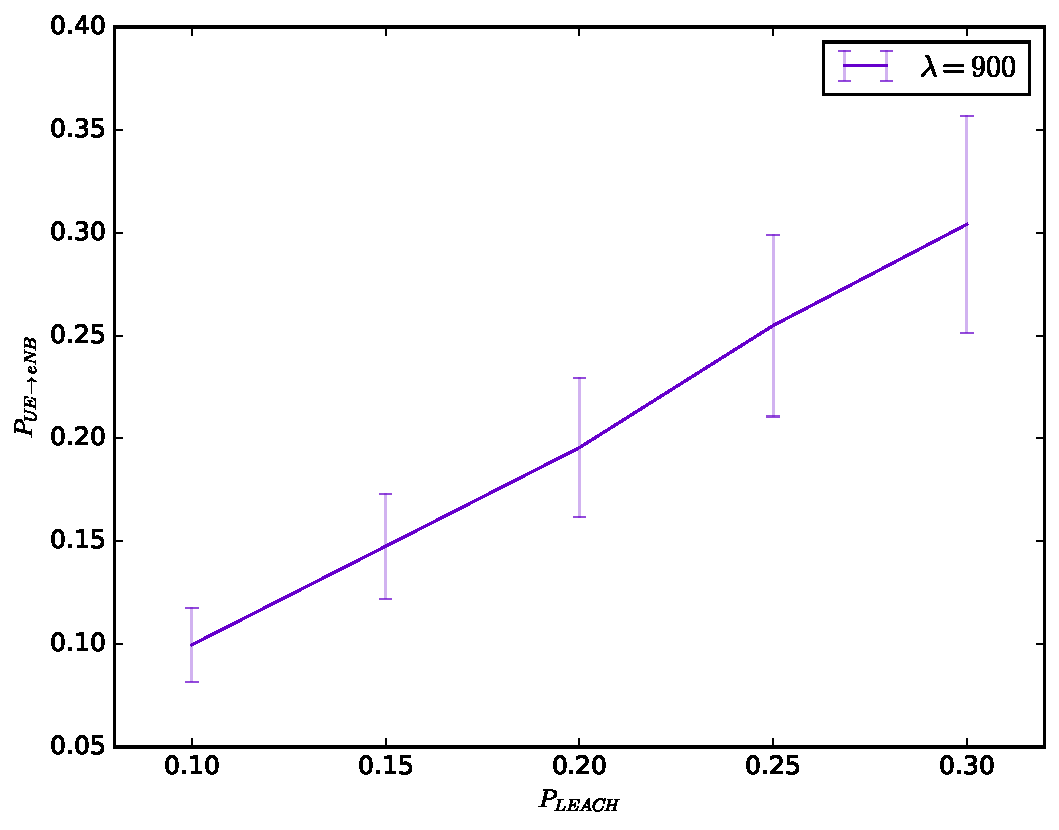
\includegraphics[width=0.6\linewidth]{figures/LEACHN_2}
% \caption{LEACH: Percentage of UEs connecting to eNB $P_{UE\rightarrow eNB}$ in relation to cluster head activation probability $P_{LEACH}$ }
% \label{fig:LEACHN_2}
% \end{figure}

Observing the \textbf{mean channel utilization rate $\overline{\varrho}_{channel}$} (figure \ref{fig:LEACHLINES_8}) is, unfortunately, not as straightforward. Despite the interesting shapes promised in figure \ref{fig:LEACH_8}, the high variance present in the data and visualized in figure \ref{fig:LEACHLINES_8} makes it impossible to take it too seriously. Despite this, $\overline{\varrho}_{channel}$ seems to experience a worsening behavior as $\lambda$ increases. Like $P_{UE\rightarrow eNB}$, it also experiences its lowest values with low device densities. 

We also consider this to be expected behavior: with very small, very ineffective clusters at low densities, the available resources are severely underutilized: clusters cannot be formed efficiently and the individual devices connect directly to the eNB. Towards higher values, it exhibits the contrary situation; very high densities mean a very high amount of available cluster heads and smaller clusters when compared to middling values of $\lambda$, making the average utilization go down, since each cluster serves fewer UEs. The highest value of $\overline{\varrho}_{channel}$ is thus achieved with a low CH activation probability $P_{LEACH} = 0.1$ and a middling $\lambda = 325$.

\begin{figure}
\centering
\captionsetup{justification=centering}
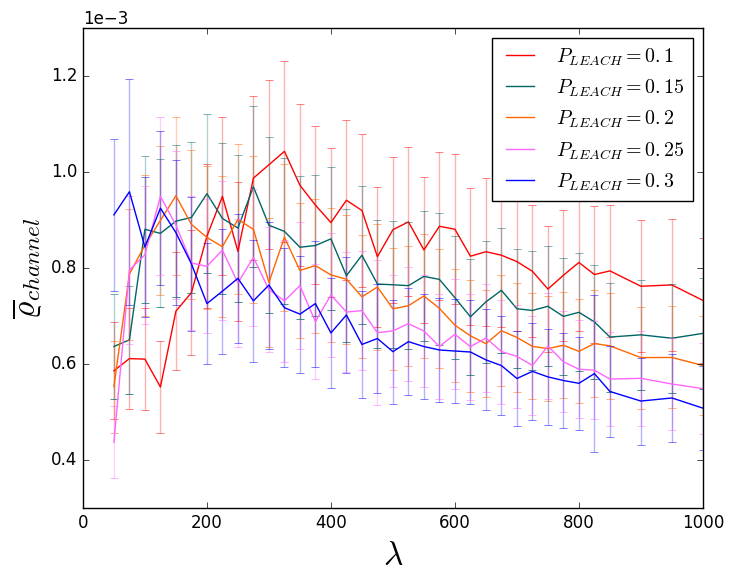
\includegraphics[width=0.7\linewidth]{figures/LEACHLINES_8}
\caption{LEACH: Mean channel utilization rate $\overline{\varrho}_{channel}$ in relation to mean point density $\lambda$ }
\label{fig:LEACHLINES_8}
\end{figure}

Moving on to \textbf{total resource efficiency} (figure \ref{fig:LEACHLINES_9}), the data seems pretty straightforward. Total resource efficiency increases with both mean point density $\lambda$ and cluster head activation probability $P_{LEACH}$. With more viable D2D connections, more devices are sharing the same pool of resources, both in time and frequency, as is explained in \ref{RE}.

While this seems to bode well for very dense networks, it is important to point out that this behavior can also be in part explained with the increase in brute D2D connection numbers that occurs with increasing values of the two variables. A more accurate measure would have to take into account the connection to the eNB with more detail, as well as the higher amount of interference caused. As mentioned earlier, this is also compounded with a mounting pressure on the resources of the eNB, which may not be able to handle both the high $\lambda$ and high resource efficiency that a simple optimization towards this measure would suggest.

\begin{figure}
\centering
\captionsetup{justification=centering}
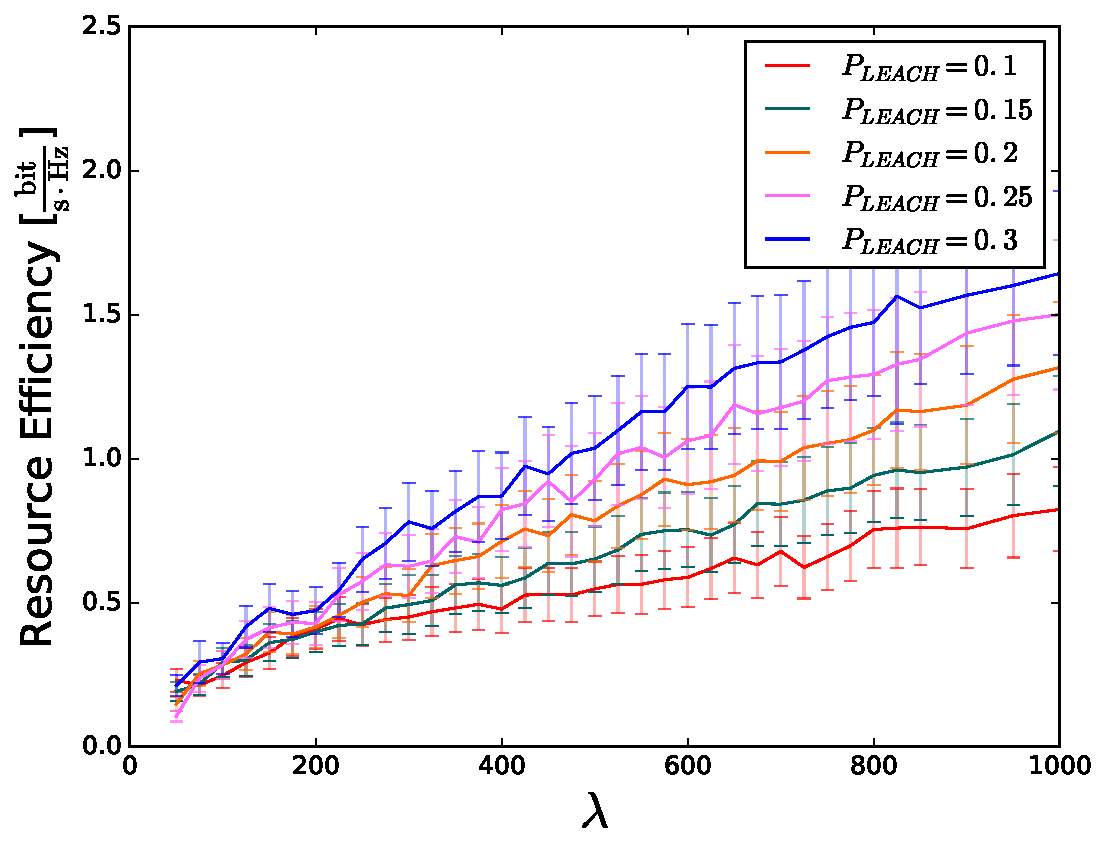
\includegraphics[width=0.7\linewidth]{figures/LEACHLINES_9}
\caption{LEACH: Total resource efficiency in relation to mean point density $\lambda$ }
\label{fig:LEACHLINES_9}
\end{figure}

Finally, we regard \textbf{mean UE drop ratio $\overline{\theta}_{drops}$} (figure \ref{fig:LEACHLINES_10}). Here, all curves present a downward trend with an increasing $\lambda$, with higher values of $P_{LEACH}$ presenting lower ones of $\overline{\theta}_{drops}$. With increasing density of devices, as well as density of cluster heads, the amount of times a UE is completely unsuccessful at connecting after 20 ``back offs'' falls to nearly 0. 

Intuitively, one might expect that $\overline{\theta}_{drops}$ would steadily rise after a period of falling, reacting to the increased interference that is caused by a large amount of devices interfering all at the same time. The explanation for this, lies again in the arrival rate of requests at the cluster head $\lambda_A$. As explained in section \ref{RAP}, the arrival rate remains constant, irrespective of the amount of UEs connected to a cluster head. An increase in density $\lambda$, which would often result in an increase in the number of devices connected thus does \textit{not} in fact cause an increase in the amount of requests. On the contrary, the amount of requests coming from a given UE in any time frame goes down when the size of its cluster grows. The negative effects of interference, though taken well into consideration, become negligible with such sparse rates of communication.

\begin{figure}
\centering
\captionsetup{justification=centering}
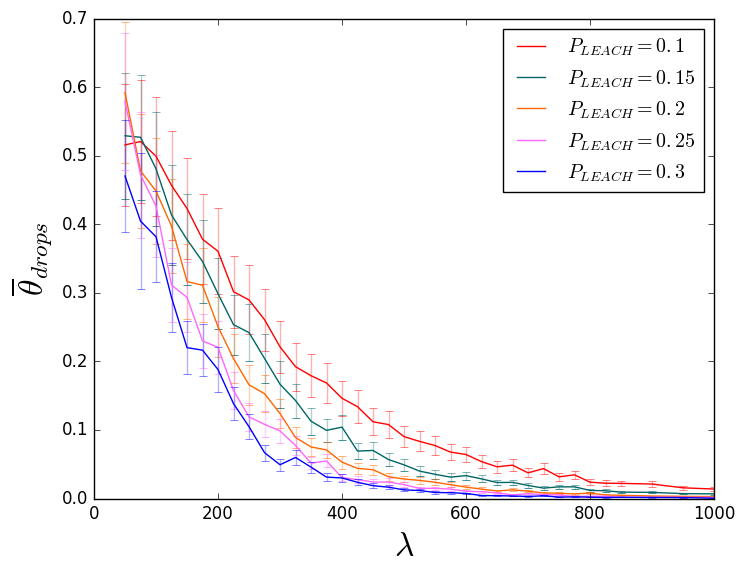
\includegraphics[width=0.7\linewidth]{figures/LEACHLINES_10}
\caption{LEACH: Mean UE drop ratio $\overline{\theta}_{drops}$ in relation to mean point density $\lambda$ }
\label{fig:LEACHLINES_10}
\end{figure}

\section{Hierarchical Algorithms}\label{description:HIERA}
\subsection{Complete-Link}\label{description:COMPLETE}

\begin{figure}
  \begin{subfigure}[b]{0.5\linewidth}
    \centering
    \captionsetup{justification=centering}
    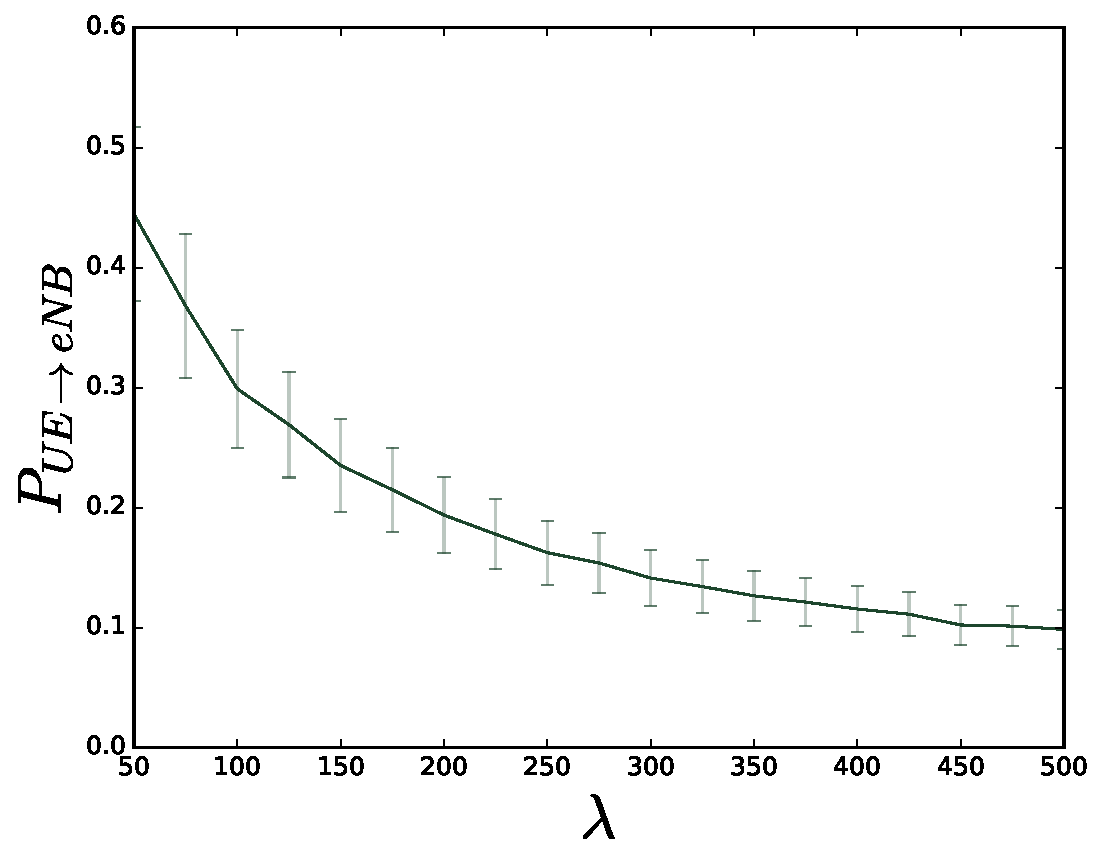
\includegraphics[width=1\linewidth]{figures/COMPLETE_2} 
    \caption{\% of UEs connecting to eNB $P_{UE\rightarrow eNB}$ }
    \label{fig:COMPLETE_2} 
    \vspace{4ex}
  \end{subfigure}%% 
  \begin{subfigure}[b]{0.5\linewidth}
    \centering
    \captionsetup{justification=centering}
    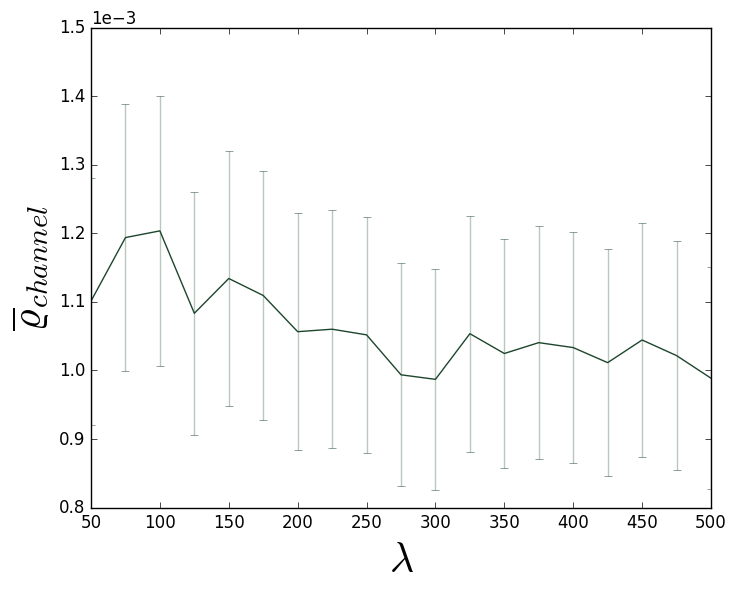
\includegraphics[width=1\linewidth]{figures/COMPLETE_8} 
    \caption{Mean channel utilization rate $\overline{\varrho}_{channel}$} 
    \label{fig:COMPLETE_8} 
    \vspace{4ex}
  \end{subfigure} 
  \begin{subfigure}[b]{0.5\linewidth}
    \centering
    \captionsetup{justification=centering}
    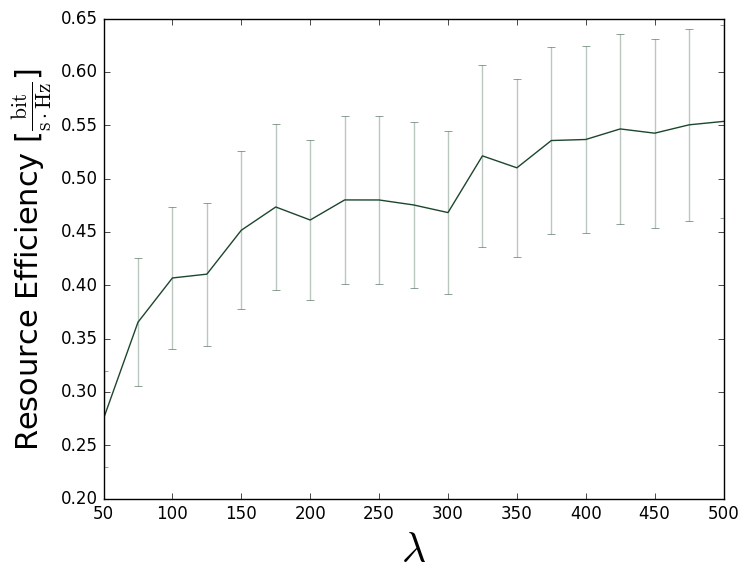
\includegraphics[width=1\linewidth]{figures/COMPLETE_9} 
    \caption{Total resource efficiency} 
    \label{fig:COMPLETE_9} 
  \end{subfigure}%%
  \begin{subfigure}[b]{0.5\linewidth}
    \centering
    \captionsetup{justification=centering}
    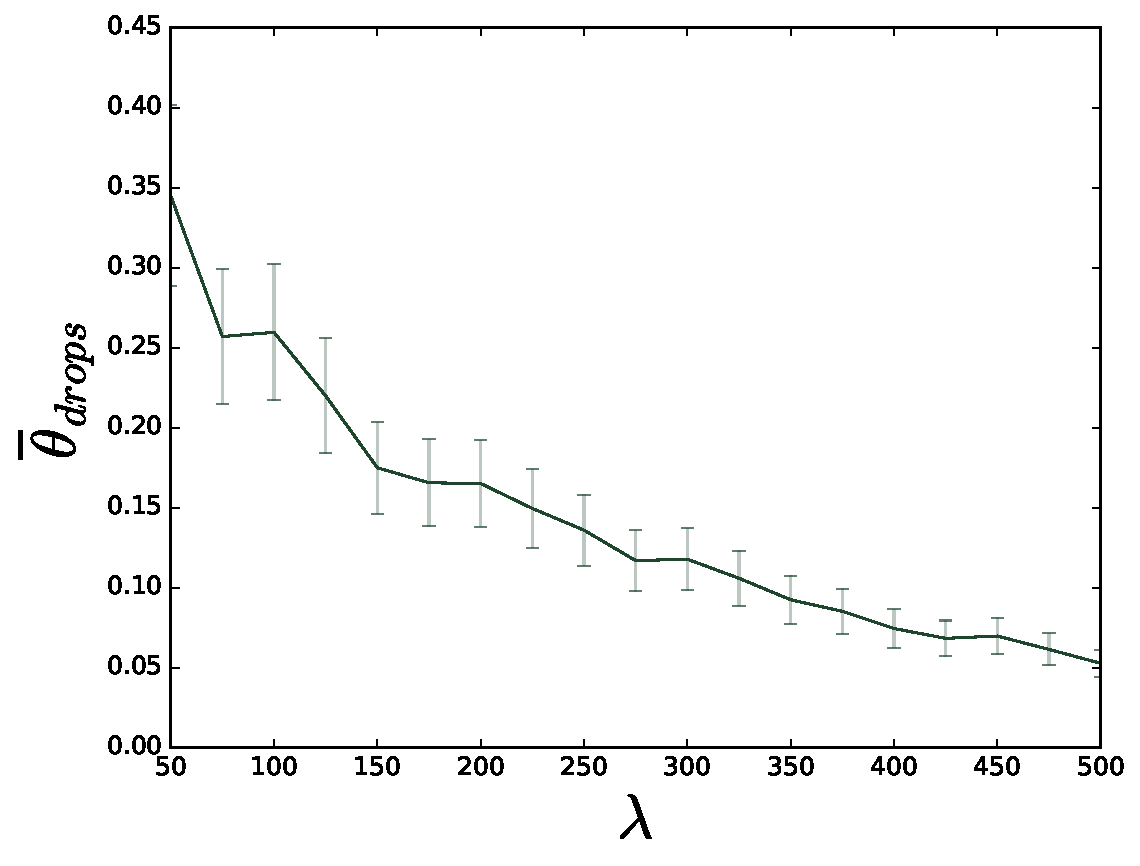
\includegraphics[width=1\linewidth]{figures/COMPLETE_10} 
    \caption{Mean UE drop ratio $\overline{\theta}_{drops}$} 
    \label{fig:COMPLETE_10} 
  \end{subfigure} 
  \caption{Behavior of Complete-Link clustering compared to $\lambda$}
  \label{fig:pretty_results_COMPLETE} 
\end{figure}

In figure \ref{fig:COMPLETE_2} concerning \textbf{percentage of UEs connecting to eNB $P_{UE\rightarrow eNB}$}, we see a steady lowering of $P_{UE\rightarrow eNB}$ towards a saturation value of around $0.1$. Unlike LEACH or Single-Link, this value is ``organic'', since the stopping criteria for the algorithm is purely the the SNR threshold previously defined. 

\textbf{Mean channel utilization rate} $\overline{\varrho}_{channel}$ (figure \ref{fig:COMPLETE_8}) shows an even weaker trend downwards than is the case in LEACH, although the high variance in the data once again restricts conclusive observations in this area. It is fair to say, however, that there does not seem to exist a strong correlation between $\lambda$ and $\overline{\varrho}_{channel}$ in this clustering scheme.

\textbf{Total resource efficiency}, in figure \ref{fig:COMPLETE_9}, experiences a stronger upswing on the lower end of the $\lambda$ axis and continues to grow throughout, albeit in a more tentative manner. The magnitude of the values stays within a similar range as LEACH, as will be further explored in section \ref{Comparison}.

Lastly, the \textbf{mean UE drop ratio $\overline{\theta}_{drops}$} plotted in figure \ref{fig:COMPLETE_10} shows an overall downward trend, as was expected from our other simulations.

\subsection{Single-Link}\label{description:SINGLE}
\begin{figure}
  \begin{subfigure}[b]{0.5\linewidth}
    \centering
    \captionsetup{justification=centering}
    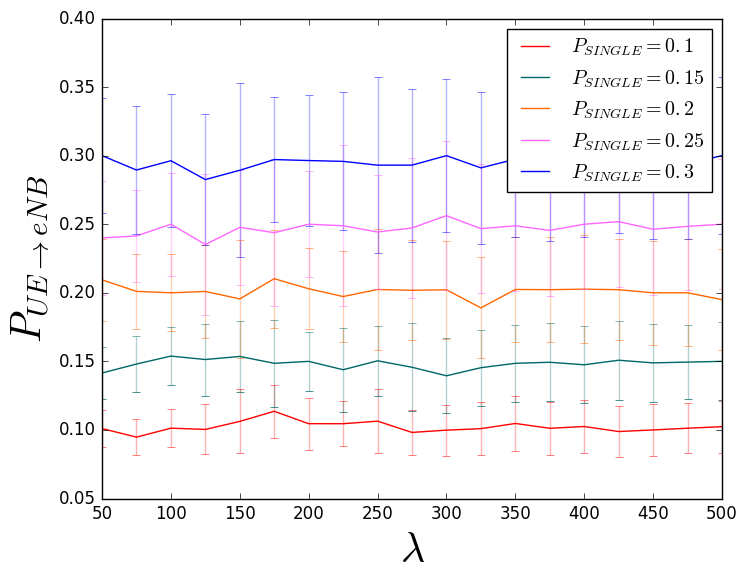
\includegraphics[width=1\linewidth]{figures/SINGLELINES_2} 
    \caption{\% of UEs connecting to eNB $P_{UE\rightarrow eNB}$ }
    \label{fig:SINGLELINES_2} 
    \vspace{4ex}
  \end{subfigure}%% 
  \begin{subfigure}[b]{0.5\linewidth}
    \centering
    \captionsetup{justification=centering}
    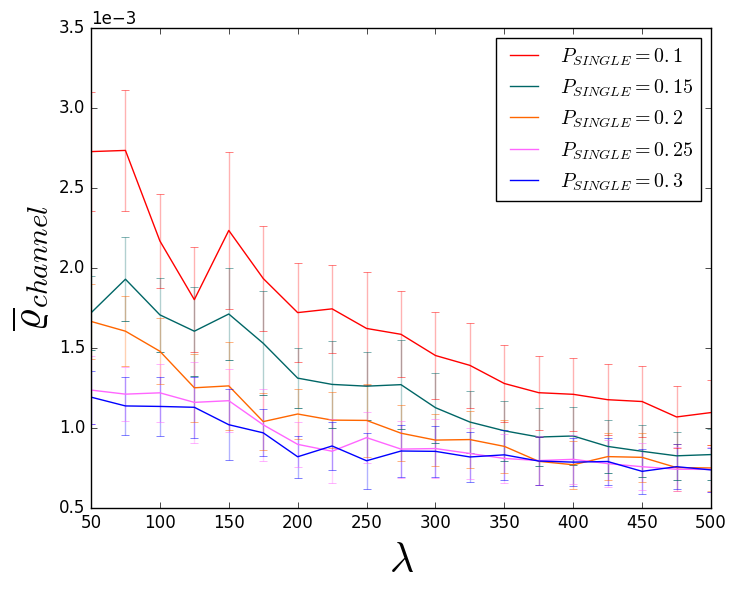
\includegraphics[width=1\linewidth]{figures/SINGLELINES_8} 
    \caption{Mean channel utilization rate $\overline{\varrho}_{channel}$} 
    \label{fig:SINGLELINES_8} 
    \vspace{4ex}
  \end{subfigure} 
  \begin{subfigure}[b]{0.5\linewidth}
    \centering
    \captionsetup{justification=centering}
    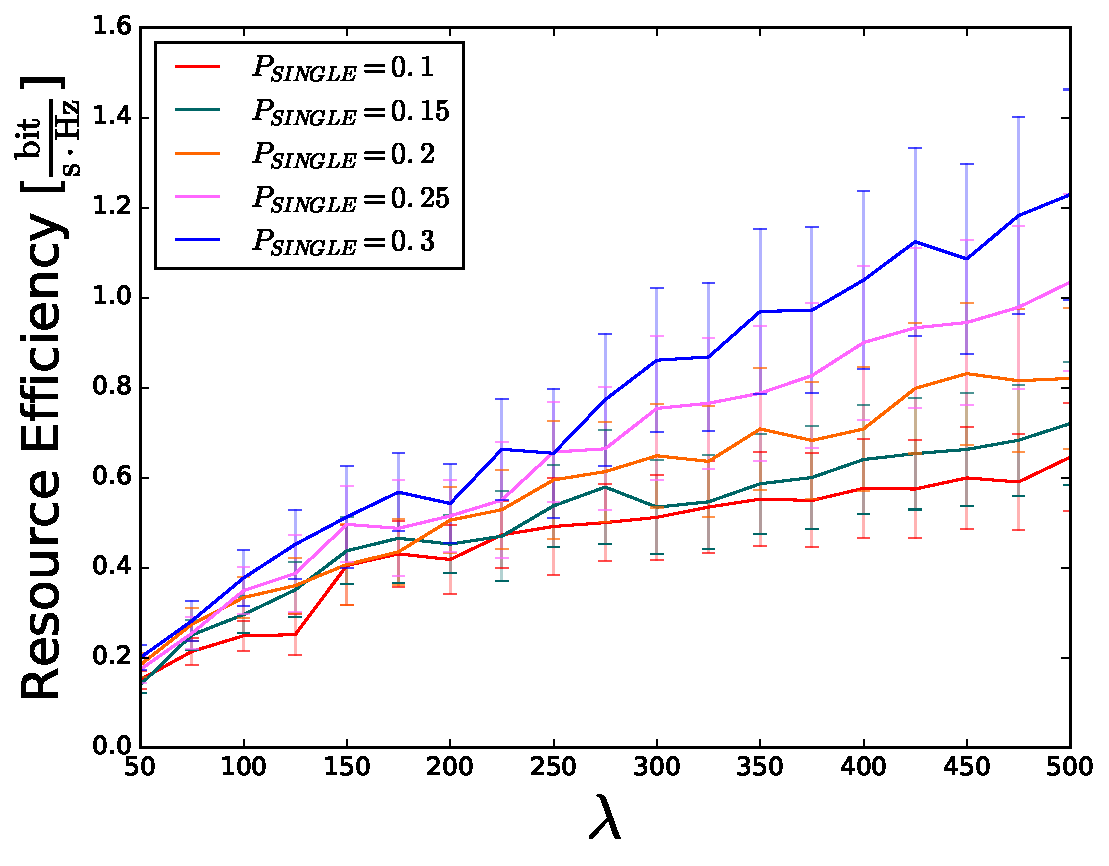
\includegraphics[width=1\linewidth]{figures/SINGLELINES_9} 
    \caption{Total resource efficiency} 
    \label{fig:SINGLELINES_9} 
  \end{subfigure}%%
  \begin{subfigure}[b]{0.5\linewidth}
    \centering
    \captionsetup{justification=centering}
    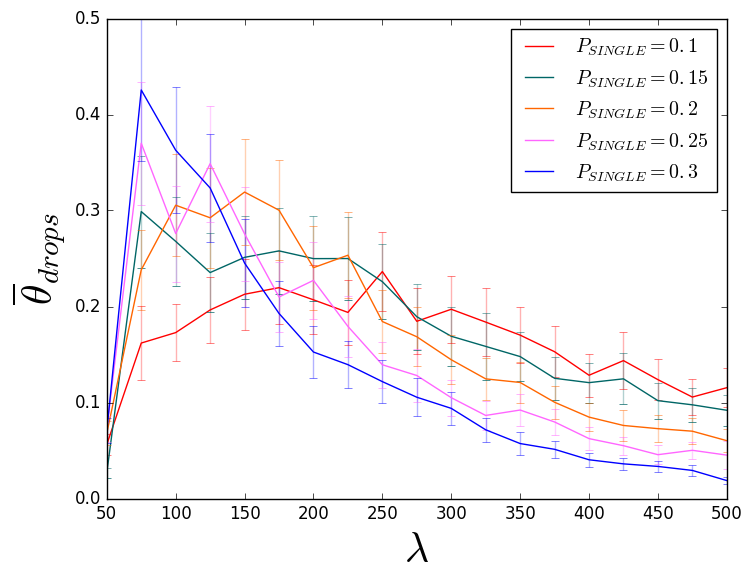
\includegraphics[width=1\linewidth]{figures/SINGLELINES_10} 
    \caption{Mean UE drop ratio $\overline{\theta}_{drops}$} 
    \label{fig:SINGLELINES_10} 
  \end{subfigure} 
  \caption{Behavior of Single-Link clustering compared to $\lambda$}
  \label{fig:pretty_results_SINGLE} 
\end{figure}

For Single-Link, we took a similar approach to that of LEACH, owing to the stark similarities between the two. As discussed in \ref{SLC}, we used the same values for $P_{LEACH}$ and $P_{SINGLE}$, both to highlight the similarities and better tease apart the differences.

It makes little sense to discuss the plot featured in figure \ref{fig:SINGLELINES_2} detailing the \textbf{percentage of UEs connecting to eNB $P_{UE\rightarrow eNB}$}. Due to the very definition of $P_{SINGLE}$ in section \ref{SLC}, it's clear that $P_{UE\rightarrow eNB}$ will remain at roughly the same level throughout all levels of $\lambda$. The fluctuations are only due to the variance of the Poisson process used to generate the positions of our UEs.

Regarding figure \ref{fig:SINGLELINES_8} and the \textbf{mean channel utilization rate $\overline{\varrho}_{channel}$}, it seems noteworthy that the variance for the metric is not as disruptive as that of earlier observations. The downward trend is clear and, as with LEACH, higher CH density roughly correlates with lower $\overline{\varrho}_{channel}$, although in this case the relationship is maintained even in lower values of $\lambda$.

\textbf{Total resource efficiency} (figure \ref{fig:SINGLELINES_9}) also exhibits a remarkably close behavior to that of LEACH. We will compare them directly in section \ref{Comparison} to disentangle the differences between both.

The \textbf{mean UE drop ratio $\overline{\theta}_{drops}$} plots of figure \ref{fig:SINGLELINES_10} TERMINAR

\subsection{Ward's Method} \label{description:WARD}

\begin{figure}
  \begin{subfigure}[b]{0.5\linewidth}
    \centering
    \captionsetup{justification=centering}
    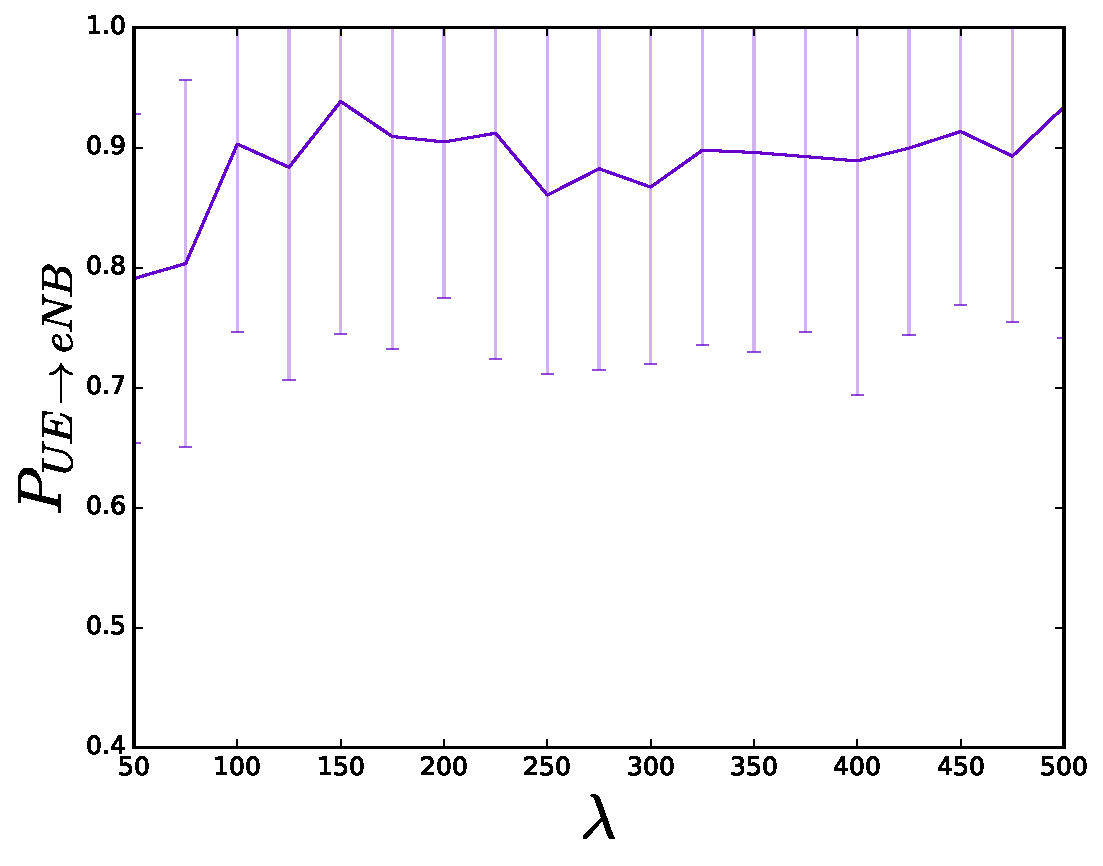
\includegraphics[width=1\linewidth]{figures/WARD_2} 
    \caption{\% of UEs connecting to eNB $P_{UE\rightarrow eNB}$ }
    \label{fig:WARD_2} 
    \vspace{4ex}
  \end{subfigure}%% 
  \begin{subfigure}[b]{0.5\linewidth}
    \centering
    \captionsetup{justification=centering}
    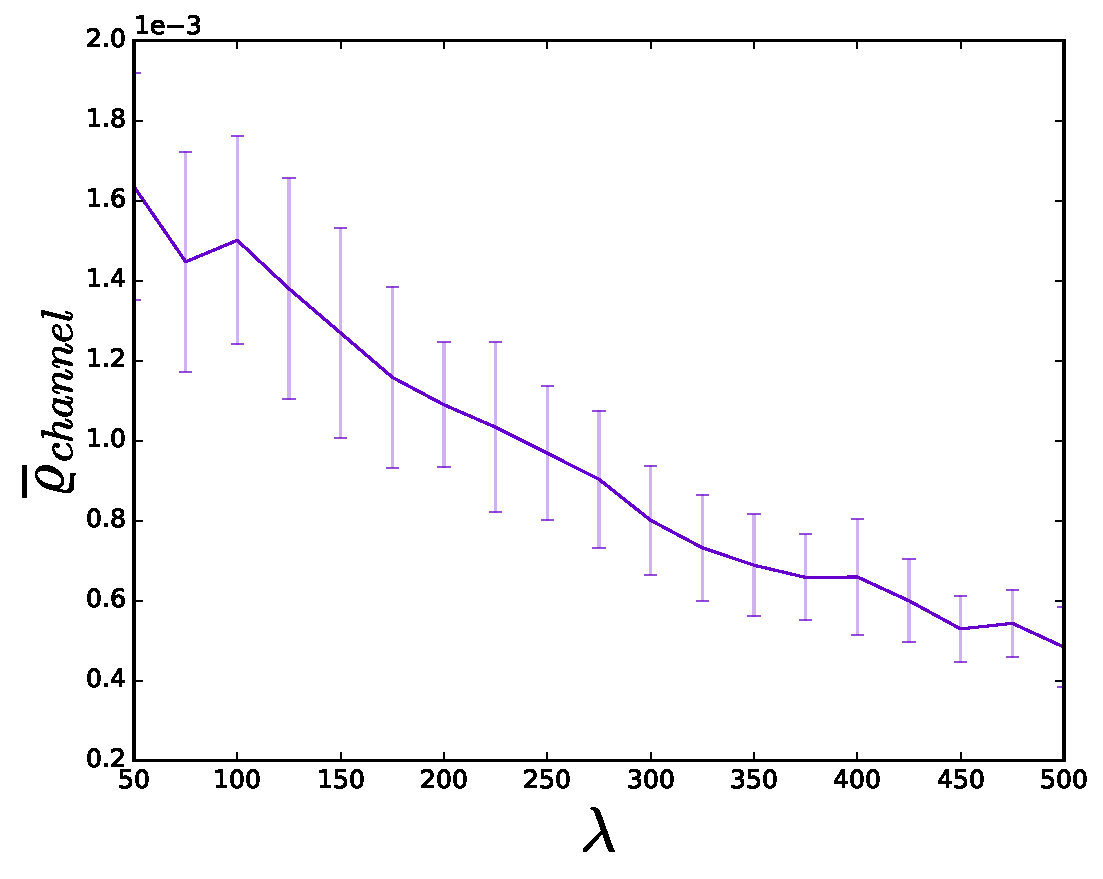
\includegraphics[width=1\linewidth]{figures/WARD_8} 
    \caption{Mean channel utilization rate $\overline{\varrho}_{channel}$} 
    \label{fig:WARD_8} 
    \vspace{4ex}
  \end{subfigure} 
  \begin{subfigure}[b]{0.5\linewidth}
    \centering
    \captionsetup{justification=centering}
    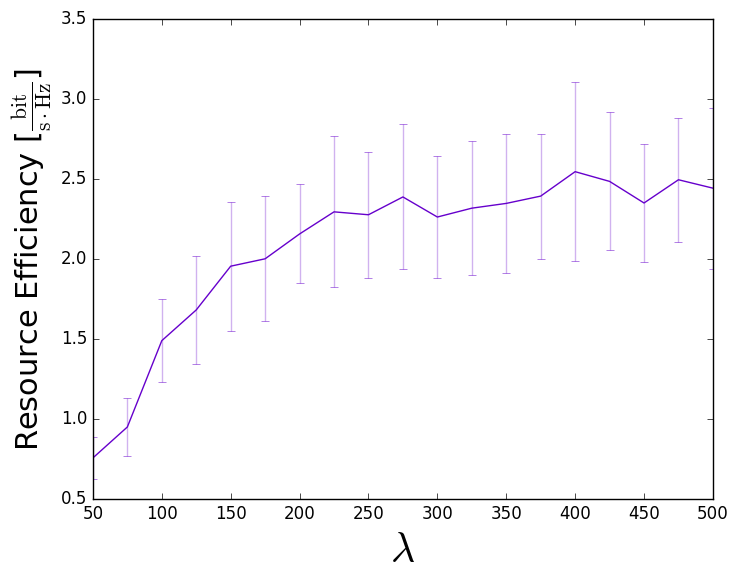
\includegraphics[width=1\linewidth]{figures/WARD_9} 
    \caption{Total resource efficiency} 
    \label{fig:WARD_9} 
  \end{subfigure}%%
  \begin{subfigure}[b]{0.5\linewidth}
    \centering
    \captionsetup{justification=centering}
    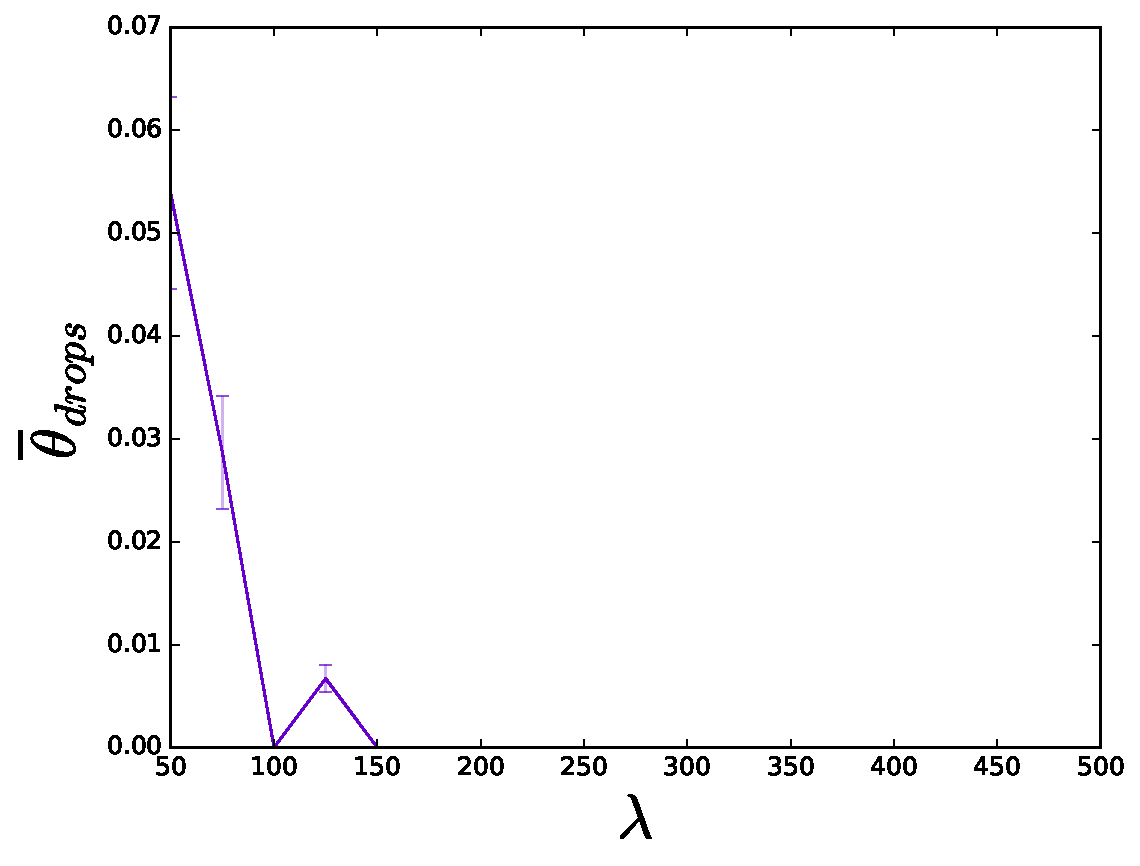
\includegraphics[width=1\linewidth]{figures/WARD_10} 
    \caption{Mean UE drop ratio $\overline{\theta}_{drops}$} 
    \label{fig:WARD_10} 
  \end{subfigure} 
  \caption{Behavior of Ward's method compared to $\lambda$}
  \label{fig:pretty_results_WARD} 
\end{figure}

Looking at the results given by Ward's method, it is immediately apparent that this was the worst clustering scheme, in terms of actually managing to provide structures to alleviate the pressure on the eNB's resources. This observation is easily explained by simply glancing at figure \ref{fig:WARD_2}, where $P_{UE\rightarrow eNB}$ is detailed. The metric hovers constantly around 90\%, meaning that the large majority of UEs are unable to be grouped into a viable cluster and elect to transmit their information through traditional means. This rate is simply unacceptable for highly dense applications like the one we are investigating.

Despite this, the few D2D connections that do exist exhibit a similar behavior than the others in terms of \textbf{mean channel utilization rate $\overline{\varrho}_{channel}$} (figure \ref{fig:WARD_8}) and \textbf{total resource efficiency} (figure \ref{fig:WARD_9}). The high magnitude of the levels of resource efficiency, although initially impressive can be easily disregarded: a very low number of D2D connections will make on average better use of all available D2D resources simply due to the fact that there are fewer elements between which to share the resource pool.

The low amount of connections is only highlighted by the bizarre \textbf{mean UE drop ratio $\overline{\theta}_{drops}$} curve of figure \ref{fig:WARD_10}. With a low number of D2D connections per cluster and, as mentioned, more resources available for each of those links, drops become a non-issue and hit 0 quickly.

\clearpage

\section{Comparison}\label{Comparison}
\subsection{Percentage of UEs connecting to eNB}
\begin{figure}
\centering
\captionsetup{justification=centering}
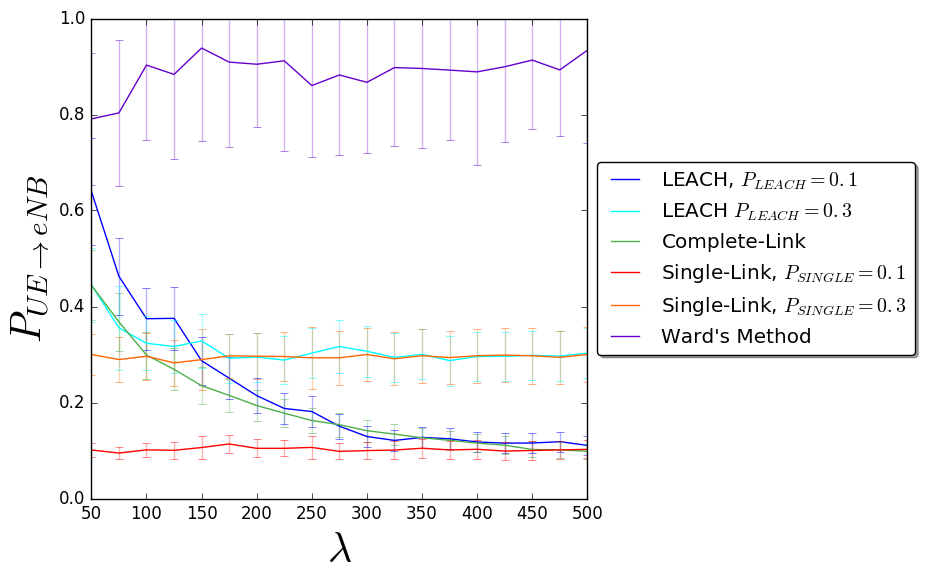
\includegraphics[width=1\linewidth]{figures/COMPARE_2}
\caption{Comparison: \% of UEs connecting to eNB $P_{UE\rightarrow eNB}$ }
\label{fig:COMPARE_2}
\end{figure}

As can be verified in \ref{fig:COMPARE_2}, most clustering schemes perform their duty of restricting the amount of connections that reach the eNB by using D2D links. The plots corresponding to Single-Link, as mentioned before, do not contain much information by themselves, but they become more intriguing when comparing them to their LEACH-spawned brethren. Lower values of $P_{LEACH}$ appear to necessitate higher densities of devices to reach their desired percentage of connections, establishing Single-Link as a better alternative when the levels of $P_{UE\rightarrow eNB}$ are of the essence and particularly in lower densities.

Complete-Link on the other hand, performs surprisingly similarly to LEACH with $P_{LEACH} = 0.1$. Despite better values of $P_{UE\rightarrow eNB}$ at lower densities, the fact that Complete-Link requires much more information from the network before it can compute clusters makes it seem more lackluster. This is only highlighted by the fact that, through most values of $\lambda$, Single-Link shows consistently lower $P_{UE\rightarrow eNB}$.

%As has been explained before, it is expected that the saturation of the different values of $P_{UE\rightarrow eNB}$ towards the end would be affected by a change in the arrival rate of requests $\lambda_A$ as more 

The easy scalability of both LEACH and Single-Link to suit a desired $P_{UE\rightarrow eNB}$
should be of note. In this way, the eNB could conceivably ``change'' algorithms depending on the load it is experiencing at a particular moment, effectively allocating available resources dynamically. This could be integrated into observations about daily data traffic patterns, restricting the desired amount of aggregated data requests in particularly busy hours and relaxing it in others.

As previously expressed in section \ref{description:WARD}, this graph particularly evidences the inadequacy of Ward's method as a clustering scheme in our simulated scenario, at least the way we defined it. It is conceivable that Ward's method could serve its purpose in situations where there is a relative wealth of available cellular resources, diminishing the need for spectrum reutilization through D2D. This scenario, however, does not correspond with either our simulations nor our expectations of the future development of wireless networking. Even then, simpler mechanisms, such as LEACH with a particularly high $P_{LEACH}$ could meet this objective without the relative complexity of Ward's method.

\begin{figure}
\centering
\captionsetup{justification=centering}
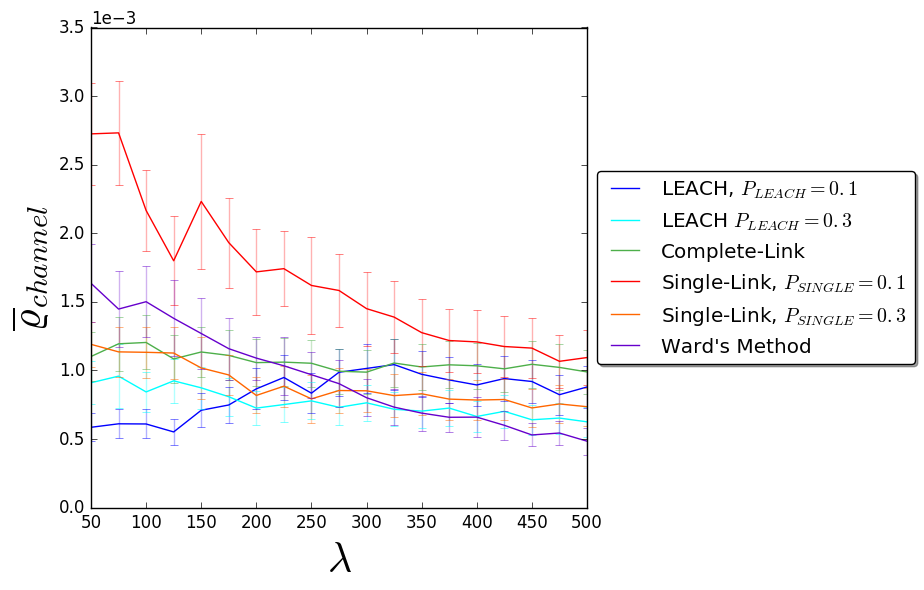
\includegraphics[width=1\linewidth]{figures/COMPARE_8}
\caption{Comparison: Mean channel utilization rate $\overline{\varrho}_{channel}$}
\label{fig:COMPARE_8}
\end{figure}

\begin{figure}
\centering
\captionsetup{justification=centering}
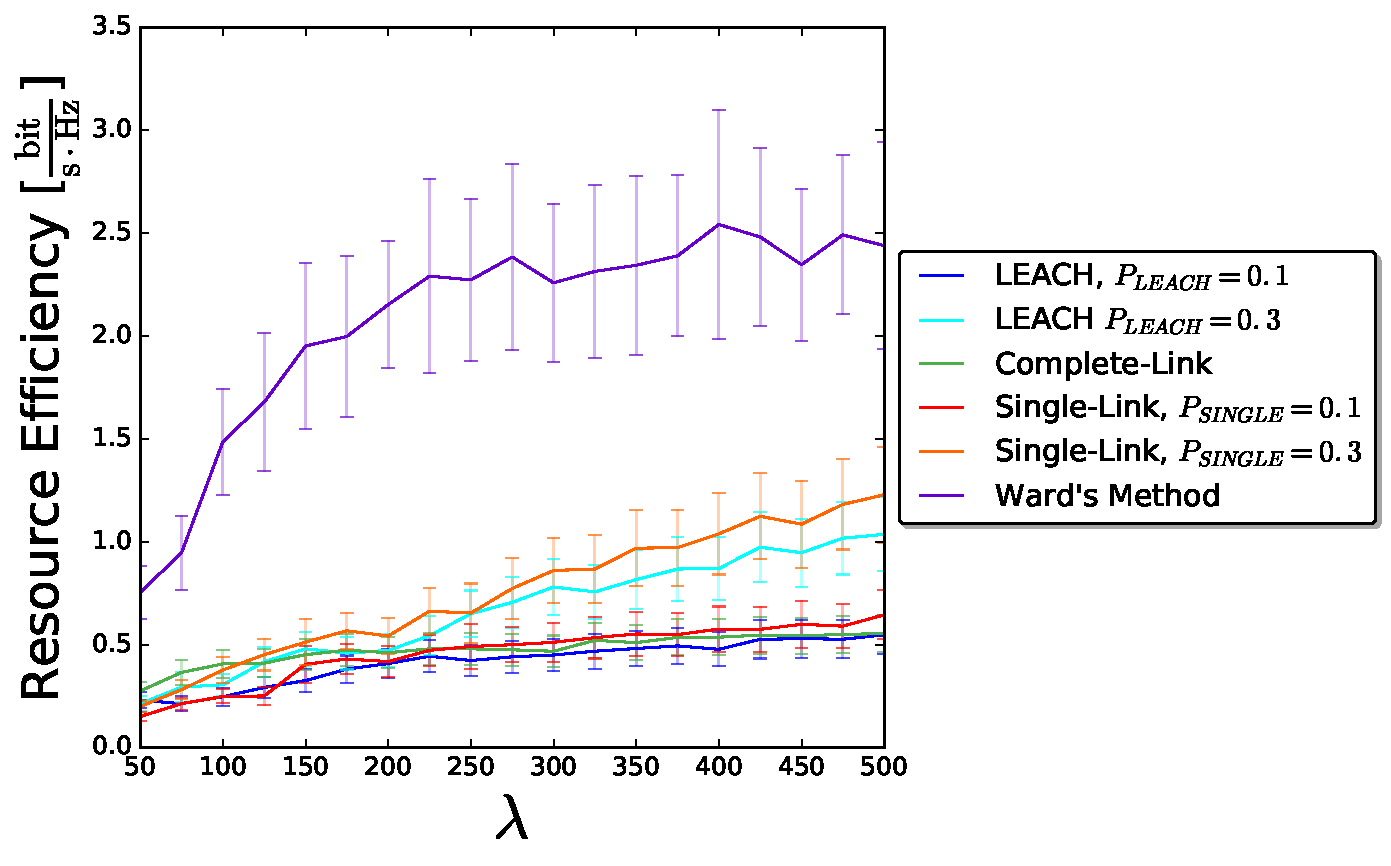
\includegraphics[width=1\linewidth]{figures/COMPARE_9}
\caption{Comparison: Total resource efficiency}
\label{fig:COMPARE_9}
\end{figure}

\begin{figure}
\centering
\captionsetup{justification=centering}
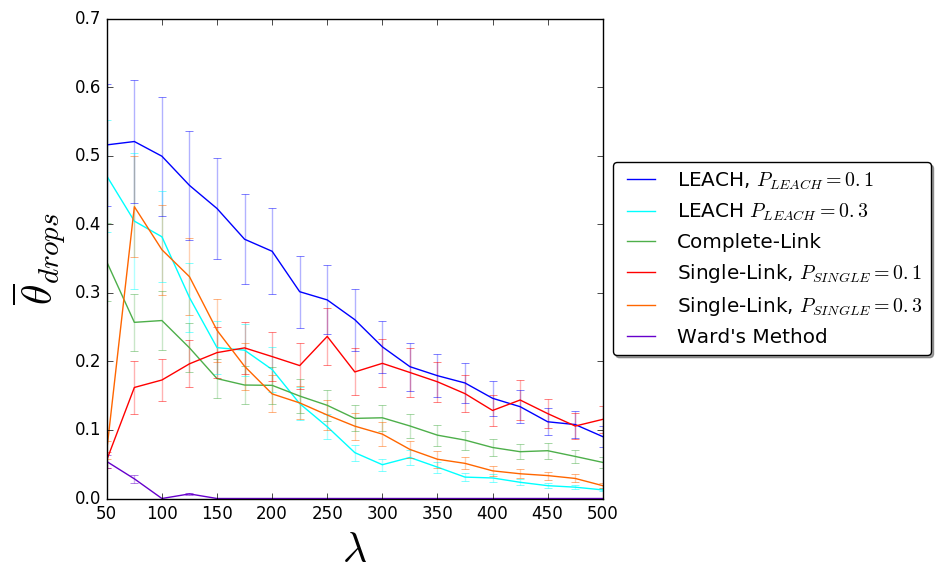
\includegraphics[width=1\linewidth]{figures/COMPARE_10}
\caption{Comparison: Mean UE drop ratio $\overline{\theta}_{drops}$}
\label{fig:COMPARE_10}
\end{figure}
